% $ platex body
% $ dvipdfmx body

\documentclass[a4j]{jarticle}

\title{「西洋音楽の歴史と理論」報告課題}
\author{KR17074 山内 拓弥}
\date{平成29年9月xx日}
\usepackage{colortbl}
\usepackage[dvipdfmx]{graphicx}
%\renewcommand{\thesection}{課題\arabic{section}}
%\renewcommand{\thesubsection}{}

\begin{document}

%\maketitle

\section{中世封建社会の解体}

\large

ヨーロッパ中世の封建社会において、
国王である主君から荘園と呼ばれる領土を与えられた領主は、
その領土の見返りとして軍事的に奉仕する契約を結ぶ。
主君が契約を破れば、臣下である領主も契約を拒否する権利があった。
また、領主は契約の内容以上に主君に尽くす義務は無かった。
このように、中世ヨーロッパの封建制は、
領主の立場が比較的強かった。
この時期、ヨーロッパで最も権力を持っていたのは、ローマ教皇であった。
しかし、1096年から1291年にわたる十字軍の遠征とその失敗により、
ローマ教皇の権威が低下した。
また、十字軍の遠征により、領主が疲弊、没落し、
国王が領主の土地を没収し、国王の権力が高まった。
14世紀頃から貨幣経済がヨーロッパにいきわたり、
余剰生産物の売却などにより農民の地位が向上した。
また、このような社会の変化に対応できずに没落した領主の土地を大商人が購入し、
新しい領主となっていった。
荘園制を基盤とする封建社会は次第に解体し、
貨幣経済と王権を基盤とする社会に変わっていく。

\section{ルネサンス時代}

中世では、文学、美術、音楽等の芸術はキリスト教中心であった。
教会の権威が弱体化すると、
芸術の中でキリスト教にかかわりの無い題材が使用されるようになり、
また、芸術活動が活発になった。
この一連の芸術運動をルネサンスと呼ぶ。
ルネサンスは13世紀にイタリアで始まった。
ダンテ(イタリア、1265-1321)は、
教会の公用語であるラテン語ではなく、
イタリアのトスカーナ地方の口語を用いて「神曲」を著した。
ボッティチェッリ(イタリア、1445-1510)は「ヴィーナスの誕生」
を製作した。
この作品は、キリスト教にとっては異教であるギリシャ神話を題材としている。
レオナルド=ダ=ビンチ(イタリア、1452-1519)
は様々な分野で作品を残しているが、
その中には精細な人体解剖図がある。
人体解剖は、教会により禁じられていた。
エラスムス(オランダ、1466-1536)は、
「愚神礼賛」を著し、その中で教会の堕落を書いた。
マキャヴェリ(イタリア、1469-1537)は、
君主は場合によっては権謀術数も必要であると主張し、
道徳や宗教とは切り離した現実的な政治学を唱えた。
コペルニクス(ポーランド、1473-1543)は、
教会が天動説を公認していた中、地動説を唱えた。
なお、レオナルド=ダ=ヴィンチによる「最後の晩餐」など、
キリスト教を題材にした作品も存在する。
フィレンチェの大商人メディチ家やローマ教皇はルネサンスを支援した。

中国で発明された羅針盤がヨーロッパに伝わり、
遠方への公開が可能となった。
この頃、東ヨーロッパはオスマン帝国が支配しており、
西ヨーロッパ諸国は、オスマン帝国を経由せずにインドと貿易する方法を模索し、
大航海時代が始まる。
1488年、ポルトガルのバルトロメウ=ディアスが、
アフリカ大陸南端の喜望峰に到達する。
1498年、ポルトガルのヴァスコ=ダ=ガマが、ついにインドに到達し、
インド航路が開かれる。
1492年、コロンブスがアメリカ大陸に到達する。
1500年、ポルトガルのカブラルがブラジルに到達する。
1522年、マゼラン一行が世界一周に成功し、世界が球形であることが実証された。

%1521
%コルテス
%アステカ王国を征服

%1533
%ピサロ
%インカ帝国を滅ぼす

%アメリカから銀がヨーロッパに流入。
%西ヨーロッパでインフレ


\section{ルネサンスの音楽}

音楽におけるルネサンス的変化は、他の分野から遅れ、
15世紀に始まり、16世紀に至る。
図\ref{fig:renaissance_summary}にルネサンス音楽の概略を示す。
15世紀初頭、現在のフランス東部にあたる地域は、
ブルゴーニュ公が支配していた。
歴代のブルゴーニュ公は戦争に明け暮れる中、
音楽や文芸に高く関心を持っていた。
ブルゴーニュ公国では、礼拝堂の音楽を担当する宮廷礼拝堂楽団が設立された。
また、別の楽団として、
主人に付き沿い、宮廷の様々な行事を音楽で盛り立てる、
ミンストレル楽団も存在した。

そのような、音楽に関心の高いブルゴーニュ公国に、
イギリス、フランス間の100年戦争のさなか、
イギリスの作曲家、ダンスタブル(1390?-1453)が滞在した。
ブルゴーニュ楽派の音楽家たちは、
3度、6度を多用するダンスタブルの作曲手法を貪欲に吸収する。
それまでのフランス音楽は、5度や8度の音程を中心とし、
それに不協和音を大胆にぶつけるという伝統があったので、
ダンスタブルの使用した3度、6度音程の柔和は響きは、
ブルゴーニュ公国の人々には新鮮に聞こえたと考えられる。

初期ルネサンス、ブルゴーニュ楽派の代表的な作曲家に、
ギヨーム・デュファイ(1400頃-1474)がいる。
デュファイの作品として、ミサ曲、モテットといった宗教音楽、
また世俗音楽のシャンソン、合わせて約200曲が知られている。
デュファイの代表的な方法として、
各楽章に同じ定旋律を用いる、
各楽章の冒頭の動機を共通にする、
という循環ミサ曲というものがあげられる。
また、ミサ曲「もし私の顔が青いなら」や「武装せる人」
に古いスタイルの聖歌ではなく、世俗曲の旋律を用い始めた。
祈りを中心としたものから、
音楽そのものを楽しむ様にミサ曲への捉え方が変化したと言える。




グーテンベルク(ドイツ、1398-1468)活版印刷を発明した。


聖ピエトロ大聖堂の大改修
贖宥状
1517 95ヶ条の論題
1521 教会から破門
プロテスタント
ルターの主張は、活版印刷によりドイツ国内に広がった。
救済は信仰によってのみもたらされる
聖書が唯一の拠り所である
神の前に万人は平等であり、信徒は全て伝道者である

カトリックのミサ典礼
聖歌は修道士や聖歌隊によって歌われる
ルター 1483-1546
礼拝に参列した会衆が共に歌って神を賛美し祈りを捧げる
ドイツ語の式文、コラールを定める

カルヴァン 1509-1564
現世での勤労と禁欲が救いをもたらす
魂の救済は神によって既に決定されており、
人間の努力では変更不可能
予定説
人々はとにかく日々の労働を勤勉に行うしかない。
当時の西ヨーロッパの新興階層である商工業者が支持

イギリス
ヘンリー8世 在位 1509-1547
王妃との離婚を認めない教皇に反発
カトリックとプロテスタントの折衷
熱心なプロテスタントの信者をピューリタンという

カトリック
対抗宗教改革
1545
トリエント公会議 1545-1563
卑猥で不純な音楽を排除すること
などが決議
複雑なポリフォニーに非難


\begin{figure}[tb]
 \begin{center}
  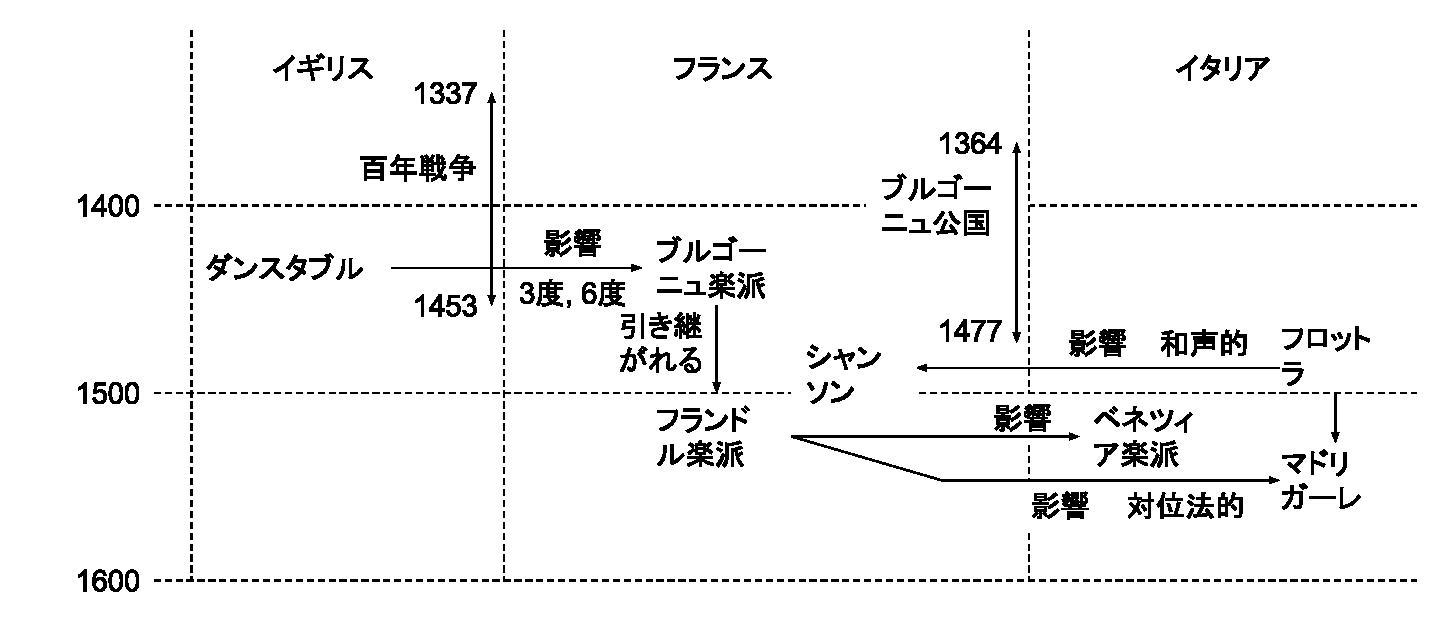
\includegraphics[width=\hsize]{fig/renaissance_summary.eps}
  \caption{ルネサンス音楽概略}
  \label{fig:renaissance_summary}
 \end{center}
\end{figure}

\begin{table}[tb]
 \begin{center}
  \caption{西ヨーロッパ中世とルネサンスの比較}
  \label{tab:comparison}
  \begin{tabular}{|l|l|} \hline
  中世                       & ルネサンス                         \\
  \hline \hline
  教皇が絶大な権力を持つ。   & 教皇の権威が低下、国王が力を持つ。 \\ \hline
  神が中心。                 & 人間が中心。                       \\ \hline
  非写実的な絵画、彫刻。     & 写実的な絵画、彫刻。遠近法。       \\ \hline
  教会による人体解剖の禁止。 & 人体解剖図が描かれる。             \\ \hline
  地球は平坦、天動説。       & 地球は球形、地動説。               \\ \hline
  和音は、神学的理論を優先。 & 和音は、人間の聴覚を優先。         \\
  5度音程が中心。            & 3度、6度のやわらかい響きを多用。   \\ \hline
  \end{tabular}
 \end{center}
\end{table}

\end{document}
